% THIS IS SIGPROC-SP.TEX - VERSION 3.1
% WORKS WITH V3.2SP OF ACM_PROC_ARTICLE-SP.CLS
% APRIL 2009
%
% It is an example file showing how to use the 'acm_proc_article-sp.cls' V3.2SP
% LaTeX2e document class file for Conference Proceedings submissions.
% ----------------------------------------------------------------------------------------------------------------
% This .tex file (and associated .cls V3.2SP) *DOES NOT* produce:
%       1) The Permission Statement
%       2) The Conference (location) Info information
%       3) The Copyright Line with ACM data
%       4) Page numbering
% ---------------------------------------------------------------------------------------------------------------
% It is an example which *does* use the .bib file (from which the .bbl file
% is produced).
% REMEMBER HOWEVER: After having produced the .bbl file,
% and prior to final submission,
% you need to 'insert'  your .bbl file into your source .tex file so as to provide
% ONE 'self-contained' source file.
%
% Questions regarding SIGS should be sent to
% Adrienne Griscti ---> griscti@acm.org
%
% Questions/suggestions regarding the guidelines, .tex and .cls files, etc. to
% Gerald Murray ---> murray@hq.acm.org
%
% For tracking purposes - this is V3.1SP - APRIL 2009

\PassOptionsToPackage{pdfpagelabels=false}{hyperref}
\setlength{\paperheight}{11in}
\setlength{\paperwidth}{8.5in} 
\documentclass{acm_proc_article-sp}
\usepackage{hyperref}
\usepackage{url}
\usepackage{mdwlist}

\begin{document}

\title{Spring XD: A Modular Distributed Stream and Batch Processing System}

% You need the command \numberofauthors to handle the 'placement
% and alignment' of the authors beneath the title.
%
% For aesthetic reasons, we recommend 'three authors at a time'
% i.e. three 'name/affiliation blocks' be placed beneath the title.
%
% NOTE: You are NOT restricted in how many 'rows' of
% "name/affiliations" may appear. We just ask that you restrict
% the number of 'columns' to three.
%
% Because of the available 'opening page real-estate'
% we ask you to refrain from putting more than six authors
% (two rows with three columns) beneath the article title.
% More than six makes the first-page appear very cluttered indeed.
%
% Use the \alignauthor commands to handle the names
% and affiliations for an 'aesthetic maximum' of six authors.
% Add names, affiliations, addresses for
% the seventh etc. author(s) as the argument for the
% \additionalauthors command.
% These 'additional authors' will be output/set for you
% without further effort on your part as the last section in
% the body of your article BEFORE References or any Appendices.

\numberofauthors{5} %  in this sample file, there are a *total*
% of EIGHT authors. SIX appear on the 'first-page' (for formatting
% reasons) and the remaining two appear in the \additionalauthors section.
%
\author{
% You can go ahead and credit any number of authors here,
% e.g. one 'row of three' or two rows (consisting of one row of three
% and a second row of one, two or three).
%
% The command \alignauthor (no curly braces needed) should
% precede each author name, affiliation/snail-mail address and
% e-mail address. Additionally, tag each line of
% affiliation/address with \affaddr, and tag the
% e-mail address with \email.
%
% 1st. author
\alignauthor Sabby Anandan
% 2nd. author
\alignauthor Marius Bogoevici
% 3rd. author
\alignauthor Glenn Renfro
\and  % use '\and' if you need 'another row' of author names
% 4th. author
\alignauthor Ilayaperumal Gopinathan
% 5th. author
\alignauthor Patrick Peralta
}
% There's nothing stopping you putting the seventh, eighth, etc.
% author on the opening page (as the 'third row') but we ask,
% for aesthetic reasons that you place these 'additional authors'
% in the \additional authors block, viz.

% Just remember to make sure that the TOTAL number of authors
% is the number that will appear on the first page PLUS the
% number that will appear in the \additionalauthors section.

\maketitle
\begin{abstract}
Spring XD is a unified, distributed, and extensible system for data ingestion,
real time analytics, batch processing, and data export. The project's goal is
to simplify the development and deployment of big data applications. This
paper discusses the motivation, architecture, and use cases for Spring XD.
\end{abstract}

\section{Introduction}

The era of Big Data has introduced many new technologies for data storage
and processing. The demand for these solutions is being driven by high
volumes of data that need to be captured and analyzed. These data sources
include (but are not limited to) mobile devices, vehicles (both autonomous
and manually operated) and large scale applications.

These large scale data processing requirements have led to the creation
of new projects such as Apache Hadoop~\cite{hadoop}, Apache Spark~\cite{spark},
and Apache Kafka~\cite{kafka}. Each of these projects was conceived
to solve a specific data processing and/or storage requirement. While some
of these projects overlap, they are often complementary -- for example,
a streaming application that collects event data in Kafka in real-time and also
stores it into Hadoop Distributed File System (HDFS)~\cite{hdfs} for batch processing.

Integrating the best of breed solutions is a challenge for developers
interested in building streaming and/or batching applications. Writing
code to glue together a custom solution imposes an upfront cost,
as well as the cost of ongoing maintenance.

Spring XD was created to help developers and system operators overcome
these challenges. Spring XD provides the following features that improve developer
productivity and operational efficiency for streaming and/or batching
data applications:
\begin{itemize*}
\item A distributed runtime environment to manage and scale streaming/batching applications
\item Out of the box integration with a plethora of technologies, both established
and up-and-coming
\item An interactive shell for creating streams or jobs without writing any Java code
\end{itemize*}

Although enterprises are interested in adopting these new technologies to
meet their data demands, they have already invested heavily in older and proven
technologies such as SQL databases and messaging systems. Spring XD includes
integrations with these technologies, thus simplifying the connection between
existing systems and newer ones.

Creating a stream in Spring XD is a simple concept for those familiar with
UNIX streams and pipes. Consider the following shell command:

\begin{lstlisting}
tail -f /tmp/log.txt | grep ERROR
\end{lstlisting}

The \texttt{tail} command will continuously display the file contents. The |
will pipe the output of \texttt{tail} to \texttt{grep}, which will filter 
out all lines that do not contain the string ERROR.

The equivalent using Spring XD looks like this:

\begin{lstlisting}
stream create -name error-filter
 -definition "tail -name=/tmp/log.txt |
 filter --expression=
 payload.contains(`ERROR') | log"
\end{lstlisting}

While this specific example will only tail a local file, a distributed 
ingestion stream that aggregates, filters, and stores log file analytics
can just as easily be created with Spring XD. See section~\ref{sec:DSL} for more
details on the Spring XD DSL.


\section{Architecture}
This section describes the internal architecture of Spring XD. The Spring XD
runtime consists of admin and container server JVM processes. The admin server
is responsible for deploying modules to containers. A module is a data
processing unit used by streams and jobs. All of these processes rely on the
Spring application context for encapsulation and life cycle management.
A pluggable messaging system is used for data transfer between modules
in a stream or job. ZooKeeper\cite{zookeeper} is used for overall coordination and process
health monitoring. (See figure~\ref{fig:architecture}.)

\subsection{Application Context}
The foundation of Spring XD is the Spring application context. The application
context is a dependency injection framework that is used to instantiate
objects along with their dependencies \cite{spring-framework-reference}.
The application context provides a consistent means of declaring dependencies
and configuration for applications written in Java. All projects in the
Spring\cite{spring} portfolio depend on the application context.

\subsection{Modules}
A Spring XD Module is a unit of data processing. A stream processing module
for Spring XD consists of one of three types: source, processor, and sink.
A stream consists of a collection of modules that define a pipeline for data.
Job modules are responsible for the execution of batch jobs. Modules are
covered in detail in section~\ref{sec:Modules}.

\subsection{Message Bus}
\label{subsec:MessageBus}
Modules require a data transport in order to transfer data. Spring XD
supports pluggable transports via a messaging abstraction known as 
the Message Bus. Spring XD includes implementations based on Redis\cite{redis}, RabbitMQ,
and Kafka. Each of the message bus implementations are provided by the
Spring Integration project.

\subsection{Containers}
A Spring XD container consists of a JVM running an application context which
loads child application contexts for modules on demand. Depending on the modules
being executed by the container, the container will also create connections to
the message bus. The container is responsible for reporting the status of its deployed
modules to the admin via Zookeeper (see subsection~\ref{subsec:Admin}.)

Spring XD supports one or more containers within a cluster. The decision criteria
for selecting the number of containers is based on capacity requirements and/or access
to specific resources.  A typical Spring XD cluster has a base set of containers
running at all times so that streams or jobs can be created, deployed or launched
as needed. A user may spin up extra containers to handle the load during peak times
and then scale back as required.

A container may be associated with one or more groups. This functionality is useful
for targeting module deployments within a stream or job to specific containers.
For example, if a set of containers within a Spring XD cluster has access to
a Hadoop\cite{hadoop} file system, that set of containers can be configured as the ``hdfs'' group.
This allows for streams that include the hdfs module to target deployment of
that module only to containers within the ``hdfs'' group.

\subsection{Admin}
\label{subsec:Admin}
The Spring XD admin server hosts a REST service used for Spring XD
administration and the orchestration of streams and jobs. While a single
admin server is required, multiple admin servers may be present in a Spring XD
system for redundancy. A single admin server will be responsible for stream
and job deployments. If multiple admin servers are present, a ``supervisor''
server will be selected via leadership election coordinated by ZooKeeper.
If more than one admin server is running, any of the admin servers
can service REST requests which helps load balancing the incoming requests.


\subsection{ZooKeeper}
Apache ZooKeeper is a distributed configuration and synchronization service.
It provides primitives required for the coordination of distributed systems.
In the case of Spring XD, ZooKeeper is used for: \begin{itemize*}
	\item Admin supervisor leadership election
	\item Centralized storage for streams and jobs definitions
	\item Centralized storage for runtime deployment properties
	\item Notification of stream/job deployments and un-deployments
	\item Tracking of containers and the modules they are hosting
	\item Notification of arriving and departing containers
\end{itemize*}
\begin{figure}[ht]
\centering
\epsfig{file=xd-architecture.eps, height=2in, width=3in}
\caption{Spring XD Architecture.}
\label{fig:architecture}
\end{figure}



\section{Modules}
\label{sec:Modules}
The four module types in Spring XD are source, processor, sink, and job. Modules
in Spring XD are defined in their own application context. This allows for encapsulation
and life cycle management for modules. Additionally, the use of an application context
enables end users to plug in their own custom modules. Spring XD uses Spring 
Integration as its foundation for implementing modules. A module is comprised of components that
implement the data processing logic and one or more connectors (known as \emph{channels})
that connect to the underlying message bus.

\par

Spring XD offers a suite of 23 sources, 24 sinks, 9 processors and 9 jobs that are ready
to use at startup.  These modules integrate with a variety of well known and popular
data stores and processing systems such as JDBC\cite{jdbc}, HDFS, MongoDB\cite{mongodb},
Spark, Kafka, RabbitMQ, Sqoop, etc.  If an existing module does not meet the needs of a
given use case, Spring XD supports custom modules.

Spring XD source and sink modules are \emph{message endpoints}
\cite{enterprise-integration-pattern-message-endpoint}
that are responsible for sending data to and receiving data from external applications
respectively. A source is the entry point for data into the stream. A sink is
the module that dispatches the stream's results to an external application or storage system.
A processor module is used to modify data transmitted from the source to sink.
Multiple processors may be chained together. Batch jobs are used to execute batch
processing steps on a set of data.

\par

\subsection{Source}
\label{sec:Source}
Source modules receive inbound data and send to downstream modules in the stream or to a batch job
which could be triggered with the data. There are two source types: \emph{poller} and \emph{event driven}.
A poller source is based on the \emph{polling consumer pattern}
\cite{enterprise-integration-pattern-pollingconsumer}.
It polls an external application (such as a web service, FTP server, database) for data at a
configurable interval. An event driven source is based on the event driven
consumer pattern \cite{enterprise-integration-pattern-eventdrivenconsumer} which
opens a port to listen for incoming data that is pushed from an external application.

\par

In the case of a source module there is an ``output'' connector channel to dispatch data
transmitted by the module to a downstream module (see figure~\ref{fig:sourcembc}.)

\par

\begin{figure}[ht]
\centering
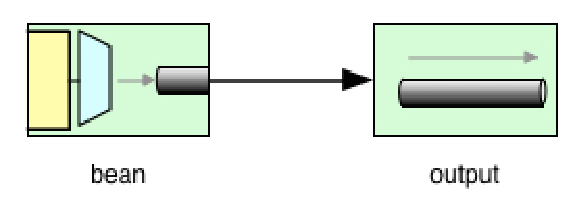
\epsfig{file=integration-module-output-channel.eps, height=.6in, width=1.75in}
\caption{Source Module Basic Components}
\label{fig:sourcembc}
\end{figure}

\par

\subsection{Processor}
\label{sec:Processor}
A processor is a module that receives data from a source or a previous processor
module's output, performs a transformation operation and sends the data
into a sink module or a downstream processor module. The basic processor
includes both ``input'' and ``output'' connector channels and the data processing component.
The input channel receives data from the upstream module and dispatches it to
the data processing component (see figure~\ref{fig:processormbc}.) It is the responsibility of
this component to transform the data. The transformed data is then sent to the downstream module
via the output channel.

\par

\begin{figure}
\centering
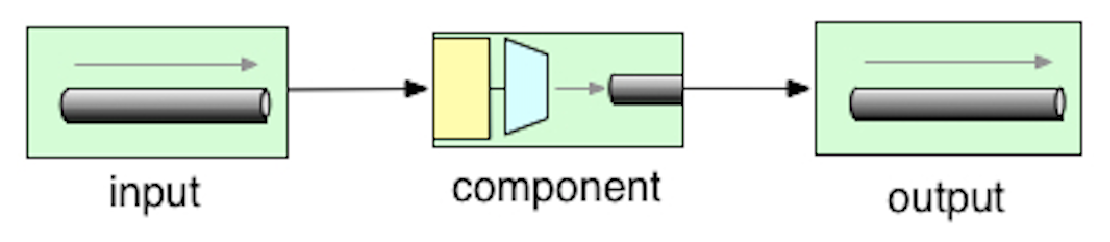
\epsfig{file=module-processor.eps, height=.6in, width=2.5in}
\caption{Processor Module Basic Components}
\label{fig:processormbc}
\end{figure}

\par

\subsection{Sink}
\label{sec:Sink}
Sink modules convert and deliver data out of the stream in a format consumable by
an external application.  There are two types of sinks: \emph{analytic} and \emph{delegate}.
An analytic sink is used to perform analytic operations (such as count, gauge) on the
incoming data and store the result into a metric repository. (See section~\ref{sec:Analytics}.)
A delegate sink translates data to the format expected by the external application.
After transforming the data, the resulting data is sent to the external application.

\par

The basic sink includes an ``input'' channel connector and a data processing
component. The input channel receives data from the stream and dispatches
it to the data processing component which is responsible for connecting to the external
application (see figure~\ref{fig:sinkmbc}.) The sinks included with Spring XD have
configurable options for retries in case of failure.

\par

\begin{figure}
\centering
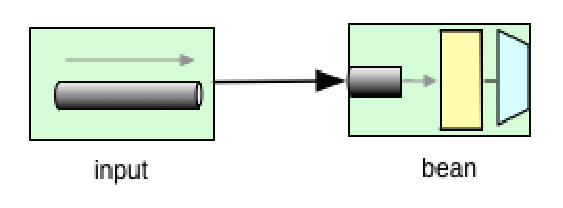
\epsfig{file=integration-module-input-channel.eps, height=.6in, width=1.75in}
\caption{Sink Module Basic Components}
\label{fig:sinkmbc}
\end{figure}

\par

\subsection{Job}
\label{sec:Job}
Spring XD uses Spring Batch \cite{spring-batch-reference}, a JSR standard (JSR-352)
for batch workload data processing as the foundation for implementing
job modules. A job enables users to execute enterprise batch processes within Spring XD.
Jobs are typically used when running long lasting tasks that have transactional requirements.
To account for failure scenarios, the workflow in the job can be designed to restart and
resume operation or roll-back the transaction altogether. A job can be triggered by a
stream with the data that act as the input to start the batch processing. This makes
streams and job modules unified under a single platform.

\par

A job typically consists of a job definition along with the supporting
data processing components as shown in figure~\ref{fig:batchmbc}.
In some cases the job definition alone is sufficient to implement the desired behavior.

\par

\begin{figure}
\centering
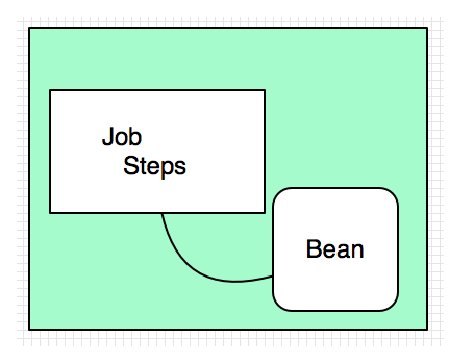
\epsfig{file=integration-batch.eps, height=.8in, width=2in}
\caption{Batch Basic Components}
\label{fig:batchmbc}
\end{figure}

\par 

\subsection{Composite}
A composite module provides a way to create a single module that contains
multiple modules. A composite module can be used to prevent
duplication when a processing chain of modules is used frequently.
Additionally, data passed between modules in a composite module will be
transmitted in memory (as opposed to the message bus) -- thus improving
performance.

\par

\subsection{Module Registry}
The module registry is where Spring XD looks for modules during
deployment. A module can be bundled as an archive or defined along with its
dependencies inside the module registry. The modules are defined in
the modules directory and are segregated in subdirectories by
type: \texttt{modules/source}, \texttt{modules/processor},
\texttt{modules/sink} and \texttt{modules/job}. The module registry is
configurable and modules may be uploaded via the admin server REST API
and Spring XD shell.
This assumes  the admin servers and containers have access to a shared 
filesystem or HDFS for the module registry
During the deployment of the module, the Spring XD runtime will load the modules
dynamically from the module registry.


\section{Processing Models}
This section describes the various processing data processing models that are possible with
Spring XD, and provides configuration and deployment examples.
Note that this is not an exhaustive list of all
deployment types, see section~\ref{sec:Use Cases} for descriptions of real
world deployments.

\subsection {Streams}

A stream defines the near-real time movement of data from a source (see~\ref{sec:Source}) to a
sink (see~\ref{sec:Sink}), passing through any number of processors (see~\ref{sec:Source}).  Spring XD streams can
also integrate with other event based solutions such as Apache Spark Streaming.

For example, the following stream definition can be used to ingest
MQTT\cite{mqtt} data sent by a number of sensors directly into HDFS:

\begin{lstlisting}
stream create ingest
  --definition "mqtt | hdfs"
\end{lstlisting}

In a more elaborate setting, an application can collect data from
different sources, and Spring XD can provide the means to merge them
in a single stream. The streams \texttt{in-mqtt} and \texttt{in-http}
collect data from sensors via MQTT and HTTP, respectively, and
contribute to a single queue \texttt{hdfs-in}. The merged result
is saved into HDFS.

\begin{lstlisting}
stream create in-mqtt --definition
  "mqtt > queue:hdfs-in"

stream create in-http --definition
  "http > queue:hdfs-in"

stream create ingest --definition
  "queue:hdfs-in > hdfs"
\end{lstlisting}

Processor modules in a stream offer the ability to transform, filter,
enrich data as it moves from one module to another.  In the example below
the stream will accept data from a http source and filter out any message
that does not have the word \emph{ocean} and then transform the message
to all caps:

\begin{lstlisting}
stream create oceanStream
 --definition "http | filter
 --expression=payload.contains('ocean') |
 transform
 --expression=payload.toUpperCase() |
 hdfs"
\end{lstlisting}

In cases that a stream should be deactivated but the definition of the stream
should be maintained, the stream can be \emph{undeployed} as shown below:

\begin{lstlisting}
stream undeploy oceanStream
\end{lstlisting}

If the stream is no longer needed it can be \emph{destroyed} as shown below:

\begin{lstlisting}
stream destroy oceanStream
\end{lstlisting}

\subsection {Batch Jobs}

Spring XD allows users to create batch workflow solutions that span traditional
use-cases such as moving data between flat files and relational databases as
well as Hadoop use-cases where analysis logic is broken up into several steps
that run on a Hadoop cluster. Spring XD can deploy and launch a Spark application
as a batch job.  The example below shows an example of creating a
job definition in XD.

\begin{lstlisting}
job create sensorProcess
  --definition "sensors"
\end{lstlisting}

(This example already assumes an existing module job named \emph{sensors} that
implements the processing logic).

An important feature of the Spring XD is the regular
execution of jobs, as well as the ability to replay older datasets, for
instance reconstructing the \emph{data views} in case of loss or error.
The following mechanisms are available:

\begin{itemize*}
\item \emph{manual} job launch through its shell user interface or
administrative UI;
\item \emph{stream-controlled} where the jobs are launched by a stream of
\emph{trigger} messages;
\item \emph{scheduled} job launch according to a \texttt{cron} expression;
\end{itemize*}

For example, a job can be launched manually as follows:

job launch sensor-process

Or, more typically, it can be launched on a schedule:

\begin{lstlisting}
stream create --name launchSensorProcess
  --definition  "trigger --cron=`0/5 * * * * *'
  > queue:job:myCronJob" --deploy
\end{lstlisting}

\subsection {Combining Streams and Jobs}

Spring XD offers the ability for streams and jobs to work together in that
a stream can launch a job or a stream can received notifications from a job
as it is executing.  In the example below an http source will pass the http
payload to the "myHttpJob, thus launching the job:

\begin{lstlisting}
stream create --name
 jobStream --definition
 "http > queue:job:myHttpJob"
 --deploy
\end{lstlisting}

In the example below a stream will receive all events from a job and write
the data to the log:

\begin{lstlisting}
job create --name myHttpJob
 --definition "httpJob"
 --deploy

stream create --name aggregatedEvents
 --definition
 "tap:job:myHttpJob >log" --deploy

job launch myHttpJob
\end{lstlisting}

\subsection {Tapping a Stream} \label{sssec:deploytap}

A tap ``listens'' to data in an existing stream and passes it into a separate
stream. The creation and existence of a tap does not modify the stream that
is being tapped. Typically the underlying message bus uses a publish/subscribe
message broker, and follows the \emph{wiretap}~\cite{wiretap}
pattern. The tapped stream is processed concurrently with the main stream, so
 consumers with different speeds downstream from the tapping point do not
 interfere with each other. Taps are recommended as way to collect metrics and perform
analytics on a stream of data. An example of this is shown below where a
tap counts the number of mqtt messages received by a source and sent to an
HDFS sink:

\begin{lstlisting}
stream create ingest
 --definition "mqtt|hdfs" --deploy

stream create ingestTap
 --definition "tap:stream:ingest>counter
 --name=ingestCounter" --deploy
\end{lstlisting}

\subsection {Module Counts and Stream Partitioning}
At deployment time a Spring XD stream can be configured to establish the number
of instances of each module in the stream. For example a stream may contain
a processor that is resource intensive, and needs to be
load balanced across multiple containers. The default
settings for a stream deployment will create one module instance for each
module in the stream definition. In the sample stream below the
deployment will create 3 data-processor instances distributed
across 3 containers in the cluster:

\begin{lstlisting}
stream create ingest
 --definition
 "mqtt | data-processor | hdfs"

 stream deploy --properties
 "module.data-processor.count=3"
\end{lstlisting}

(By default XD will send messages to each of the \emph{data-processors}
using round robin logic.)

Spring XD Streams can be partitioned at deployment time to route messages to the
same module instance based on the contents of the message. One example
would be if the processor aggregates data by sensorId and this step needs to
run using co-located resources.  An example of this is enumerated below:

\begin{lstlisting}
stream create ingest
 --definition
 "mqtt | data-processor | hdfs"

stream deploy --properties
 "module.jms.producer.partitionKeyExpression=
 payload.sensorId,
 module.data-processor.count=3"
\end{lstlisting}

In this example, instead of round robin processing by the \emph{data-processor}
module, the data passing through the stream will be partitioned by ``sensorId''
across the \emph{data-processor} modules.

\subsection {Reactive Processing}


\emph{Reactive programming} is a programming paradigm centered around asynchronous
stream processing. The central concept is that incoming data can be processed in an
ordered, asynchronous and event-driven manner, using functional operators to describe
transformations that apply to an entire stream of incoming data. Operators can
vary from individual item transformations, to grouping and aggregation over given
time windows, and can be composed into complex data processing pipelines that produce
outbound streams of data.

ReactiveX~\cite{reactivex} is one of the most common set of reactive APIs, centered around
the \texttt{Observable} abstraction of an unbounded stream of asynchronous events,
together with a rich set of operators for composing and transforming them.
RxJava~\cite{rxjava} is the Java implementation of the ReactiveX API.

Spring XD provides support for reactive programming through a special type of
processors that describe the transformations on asynchronous streams of data, as
opposed to focusing on the transformations that occur on discrete events. For example,
an RxJava processor for calculating average values over a sliding time window can look as follows:

\begin{lstlisting}
public class MovingAverage
  implements Processor<Tuple,Tuple> {

  @Override
  public Observable<Tuple>
    process(Observable<Tuple> inputStream) {
    return inputStream
      .map(tuple -> tuple.getDouble("measurement"))
      .window(5,1,SECONDS)
      .flatMap(data -> average(data))
      .map(avg -> tuple().of("average", avg)));
    }
}
\end{lstlisting}

The custom module implements the \texttt{Processor} interface and the
\texttt{process} method, whose role is not to execute transformations
on the individual messages of the stream, but to describe a series of
transformations that will be performed on the items emitted by the
\texttt{Observable}: mapping, windowing and the average calculation.

As shown in \ref{fig:rxjava}, Spring XD has the responsibility of transforming the
flow of discrete messages arriving on a processor's input channel into an
RxJava \texttt{Observable}, as well as transforming the \texttt{Observable}
returned by the processor module into a flow of discrete messages sent on
the output channel.

\begin{figure}[ht]
\centering
\epsfig{file=rxjava.eps, width=3in}
\caption{Reactive module using RxJava}
\label{fig:rxjava}
\end{figure}

For example, the processor listed above can then be packaged as part of a regular
 processor module (called, for example \emph{averages}) and uses as part of a
 regular stream definition.

\begin{lstlisting}
stream create --name average-sensors
  --definition  "mqtt | averages | log" --deploy
\end{lstlisting}


\section{Use Cases}
\label{sec:Use Cases}

The following customer use cases are being supported in the field by the
Spring XD team.

\subsection{Fault Detection}
\textit{Challenge}: A large equipment manufacturer is interested in
ingesting machine data to apply predictive analytics to proactively monitor
performance and adjust business operations.

\textit{Solution}: Given the extensible architecture in Spring XD, a custom
source module is created to handle proprietary data formats, thus allowing
consumption and transformation of data complying with their proprietary
standards. The predictive models, complying with PMML specification, were
generated based on historical trends. Spring XD's analytic-pmml processor is
used in a stream to intercept machine events to compute predictions in
real-time. The outliers were captured in Redis\cite{redis} for dashboard alerts 
and ad-hoc data analysis via REST.

\subsection{Enterprise Modernization}
\textit{Challenge}: A large retail provider is heavily invested in the Hadoop
\cite{hadoop}
ecosystem. They weren't keen on maintaining or supporting several products in
production - operationalization is painful. They want to streamline and
modernize their Hadoop workflows.

\textit{Solution}: As one-stop runtime, Spring XD provides dozens of data
integration adapters to send and receive data from external applications, thus
allowing the customer to use the unified approach for all ingestion use-cases.
Building upon Spring Batch, Spring XD also provides multiple batch jobs for data movements along with granular workflow steps. This further eliminated the need for relying on different workflow and data movement tools. Whether it is MapReduce, Hive, Pig, or HBase scripts - the developer experience is the same in Spring XD.

\subsection{Data Ingest}
\textit{Challenge}: A startup in San Francisco is looking for a solution to
unify stream and batch operations. 

\textit{Solution}: Spring XD is used as a standard tool for ingesting data 
into Hadoop . Whether it is real-time (i.e., online) or batch 
(i.e., offline),
the out of the box fixtures delivered immediate benefits. Overall, the data
integration, orchestration, and data movement capabilities were handled end
to end by Spring XD.

\subsection{24/7 Production Pipelines}
\textit{Challenge}: A large IT enterprise wants to build data pipelines to
monitor current software and hardware sales in order to predict and forecast.
Building pipelines is one; running them reliably 24/7 with strict SLAs is
another big challenege.

\textit{Solution}: Spring XD is built as highly-available runtime. Automatic
recovery from fault scenarios along with reprocessing of data events fulfilled
SLAs guarantees. Production running pipelines in Spring XD are long running
processes. For ad-hoc operations such as querying, machine learning, or
data crunching, `taps' in Spring XD were adopted to fork the data from primary
pipeline. This results in no disruption with the primary pipeline, at the
same time satisfying ad-hoc demands.

\subsection{Closed-loop Analytics}
\textit{Challenge}: A finance institution wants to build a platform to detect
fraudulent transactions. They had years of historical data in varying formats
and the transactions happening in real-time, at high volume. They want to
automate generation of historical models from raw dataset and apply the models
to real-time events. No in-house talent to build one; neither had the budget to buy expensive products.

\textit{Solution}: A batch job is used to learn from historical data to
produce predictive models complying with PMML specification. A step
in the batch workflow is orchestrated to deliver the generated models to
streams for real-time predictions. The predictions were persisted
on in-memory data stores to visualize the data via dashboard. Spring XD eliminates top-talent hires to operationalize data analytics pipeline.


\section{Related Work}
This section compares and contrasts Spring XD to similar projects.

\subsection{Spring XD and Spark}
Spark is a general-purpose framework for large scale data processing.

For customers who need a rock solid ingestion platform based on mature open source technology, analytical stream APIs for the 80 percentage use case, RESTful control over stream processing and batch jobs across a range of big data technologies, as well as simplifying development and testing of Spark applications, Spring XD is available and supported today.

The following features differentiate Spring XD and Spark Streaming.

\begin{itemize*}
\item Reliably operate 24/7.
\item Ingest data into HDFS following to best practices (no small files) and with zero code.
\item Microbatching based on event count.
\item One event at a time processing.
\item Specify specific hosts where calculations are performed.
\item Decouple infrastructure code from business logic\slash analytics.
\end{itemize*}

The following features differentiate Spring XD and Spark Batch processing.

\begin{itemize*}
\item Provider a REST API and lifecycle management of Spark jobs.
\item Integrate with other Batch systems.
\end{itemize*}

In the future Spring XD will continue to provide additional integration with Spark features such as MLLib and SparkSQL.

\subsection{Spring XD and Storm}
Storm is a distributed computation system for real time stream processing.

For customers who are in need of real time stream processing, distributed data computations, and ETL capabilities, Spring XD as an unified runtime supports variety of use cases ranging from classic enterprise to Big Data and IoT. 

The following features differentiate Spring XD and Storm.

\begin{itemize*}
\item Spring XD's Shell compared with Storm's API programming paradigm delivers immediate productivity. No coding, IDE, bundling or packaging necessary. The high level DSL abstracts complexities through developer friendly fixtures.
\item REST APIs allows topology to be built in isolation without having to disrupt existing pipelines.
\item Loosely coupled `modules' that are responsible for ingestion, analytics, data processing, machine learning or data export can be individually managed and dynamically scaled.
\item Simplified governance model for `modules' (unit\-of\-work) and colocation capabilities.
\item Composition of `modules' (unit\-of\-work) improves performance characteristics. 
\item Building upon the reactive streams specification, customers have the option to choose from Spring Reactor, Spark Streaming or RxJava functional APIs, to build complex data centric applications.
\end{itemize*}

Spring XD provides you the right tool for the job, not forcing unnecessary complexity while remaining open and extensible.

\subsection{Spring XD and Flume}
Flume is a distributed system for collecting, aggregating and moving large data sets. 

For customers who need collecting and moving data, Spring XD simplifies lifecycle management, coordination, and automation of data pipelines. A high level DSL is all you need to operationalize data movements. 

The following features differentiate Spring XD and Flume.

\begin{itemize*}
\item Nothing manual and no coding! The high level DSL abstracts configuration and setup. One line DSL declaration automates data collection, processing, and export to a desired format or destination.
\item Manage data centric workflows with REST APIs either via DSL, admin ui, or custom applications.
\item Administer or monitor data pipelines through the UI, Jolokia or JMX endpoints. 
\item >500 combinations of data pipelines/flows can be created OOTB.
\item Granular control options to intercept step execution of data pipeline to create complex data driven workflows.
\item Flexibility through `Deployment Manifest' to declaratively configure data partitioning strategy to route data to a specific consumer instance in the cluster. Improves performance characteristics by virtue of colocation.
\end{itemize*}

No more config files, IDE, bundling, packaging or deploying artifacts. Spring XD's developer friendly fixtures deliver productivity. Flume offers HBase, Solr, and ElasticSearch sinks along with encryption support for Avro sources, which we are planning to address in our future releases.

\subsection{Spring XD and Oozie}
Oozie is a workflow scheduler engine to manage Hadoop workloads such as MapReduce or Pig jobs. 

For customers who need workflow or a coordinator engine, Spring XD, as a unified platform provides orchestration of directed graph processes to govern not just Hadoop but any data workflows. 

The following features differentiate Spring XD and Oozie.

\begin{itemize*}
\item Building upon Spring Batch, a JSR standardization (JSR-352) of batch workload data processing, Spring XD inherits rich enterprise features and customer trust.
\item Ready to use frequently used workflow jobs such as file-to-jdbc, file-to-hdfs, ftp-to-hdfs, hdfs-to-jdbc, hdfs-to-mongo, jdbc-to-hdfs, spark-job, and sqoop-job.
\item Flexibility to create custom workflow jobs through REST APIs.
\item Dynamic scaling of OOTB workflow-jobs and custom-workflow-jobs without having to bring down the runtime cluster or the currently running topology.
\item Runtime offers bidirectionality between real-time streaming and offline batch workflows to accommodate complex data processing use cases.
\item Ability to create and launch workflow-jobs from admin ui. Historical snapshots of execution, errors and states are available for exploration via admin ui.
\item Portable runtime that can run where there is JVM. On-prem, Pivotal CloudFoundry, YARN, Mesos, Docker or EC2.
\end{itemize*}

Bridging the gaps between offline and near real time data, Spring XD will continue to evolve as one stop platform for data workflows to efficiently process the data in-transit, at-rest, and in-use. Oozie offers HCatalog integration, which we are planning to address in our future releases.

\subsection{Spring XD and Sqoop}
Sqoop assists with data transmission between Hadoop and relational databases.

For customers who need data ingest and export between various databases and Hadoop, Spring XD's unified platform facilitates out of the box fixtures to orchestrate data movements reliably. 

The following features differentiate Spring XD and Sqoop.

\begin{itemize*}
\item Comprehensive lifecycle management platform for not just data transmission between Hadoop and Databases but also real time data ingest, analytics and export use cases.
\item Extending the workflow infrastructure to write custom tasklets is straightforward.
\item Simplified linux style semantics to create, deploy and destroy data pipelines.
\item Flexibility to introduce custom data pipelines through REST APIs.
\item Unified functional programming runtime to support reactive streams specifications. Either Spring Reactor, Spark Streaming or RxJava functional APIs can be used to build reactive data pipelines.
\end{itemize*}

Sqoop offers data validation, data merge, incremental data imports, and HCatalog integration among others. As a unified platform, Spring XD provides an OOTB Sqoop job to take advantage of the features at the same time also efficiently orchestrate lifecycle of data workload use cases efficiently. We will also be able to leverage 


\section{Conclusion}

Mission critical data applications cannot live in a vacuum. The abundance of data
and specialized applications to process and store it require a holistic approach.
Spring XD is a formidable solution for managing the data flow and processing
between these applications. Spring XD integrates with systems ranging from decades
old RDBMS to cutting edge Big Data. The suite of Spring Framework projects that
Spring XD builds upon allows for flexible extensibility. The distributed runtime
built on ZooKeeper provides reliability and scale out capabilities for streams
and jobs. 


%\end{document}  % This is where a 'short' article might terminate

%ACKNOWLEDGMENTS are optional
\section{Acknowledgments}
This section is optional; it is a location for you
to acknowledge grants, funding, editing assistance and
what have you.  In the present case, for example, the
authors would like to thank Gerald Murray of ACM for
his help in codifying this \textit{Author's Guide}
and the \textbf{.cls} and \textbf{.tex} files that it describes.

%
% The following two commands are all you need in the
% initial runs of your .tex file to
% produce the bibliography for the citations in your paper.
\bibliographystyle{abbrv}
\bibliography{spring-xd}  % sigproc.bib is the name of the Bibliography in this case
% You must have a proper ".bib" file
%  and remember to run:
% latex bibtex latex latex
% to resolve all references
%
% ACM needs 'a single self-contained file'!
%

% This next section command marks the start of
% Appendix B, and does not continue the present hierarchy
\balancecolumns
% That's all folks!
\end{document}
